\section{Aufbau und Durchführung}
\label{sec:Durchführung}
Zur Messung des Elastizitätsmoduls werden jeweils 4 Messreihen für den runden und den quadratischen Stab durchgeführt.
Zu beginn wurden die Maße der Stäbe aufgenommen, um deren Dichten zur Bestimmung des Materials zu erhalten und den Querschnitt
für die Berechnung zu bestimmen. Für die folgenden Messverfahren wird ein Aufbau \autoref{fig:MessApp} entsprechend verwendet.
\begin{figure}[H]
    \centering
    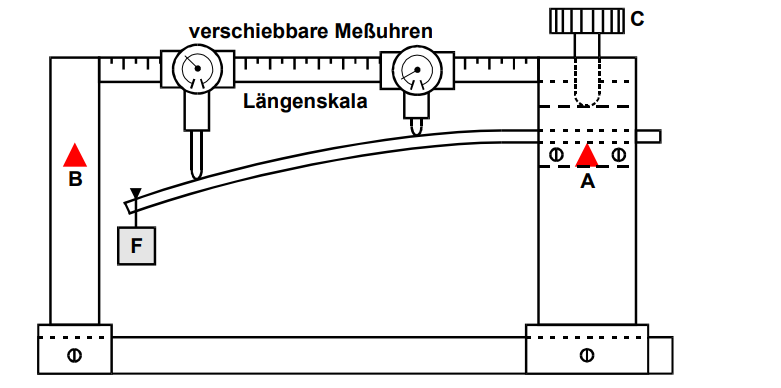
\includegraphics[scale=1]{content/MessApp.png}
    \caption{Messapperatur}
    \label{fig:MessApp}
\end{figure}
\subsection{Einseitige Einspannung}
\label{subsec:EinseitigeEinspannungAuD}
Bei der einseitigen Einspannung werden die Stäbe wie in \autoref{fig:MessApp} an A eingespannt und zunächst eine Nullmessung, also
eine Messung ohne angehängtes Gewicht F, für beide Stäbe durchgefürt und Werte $D_0(x)$ mit der rechten Messuhr in gleichmäßigen Abständen gemessen.
Anschließend wird \autoref{fig:MessApp} entsprechend das Gewicht F angehängt, welches so gewählt wird, dass die Auslenkung $D(x)$
aus der zuvor bestimmten Ruhelage zwischen $3\unit{\milli\meter}$ und $7\unit{\milli\meter}$
liegt, denn über $7\unit{\milli\meter}$ verhalten sich die Stäbe nicht mehr elastisch. Es werden Werte $D_M(x)$ in den gleichen Abständen wie bei der Nullmessung aufgenommen,
aus denen die Auslenkungen $D(x) = D_M(x) - D_0(x)$ berechnet werden.
\subsection{Beidseitige Auflage}
\label{subsec:EinseitigeEinspannungAuD}
Es wird für die beidseitige Auflage der Stäbe auch die Apperatur aus \autoref{fig:MessApp} verwendet und der Stab nur an den Stellen A und B aufgelegt.
Zu beginn wird wie bei der einseitigen Einspannung eine Nullmessung von $D_0(x)$ für beide Stäbe durchgeführt, nur das hierbei zwischen rechts und links vom
Mittelpunt der Stäbe unterschieden wird. Das Gewicht F wird hierbei anschließend in der Mitte des Stabes aufgehängt und groß gewählt, da die Auslenkung $D(x)$
sonst sehr klein sind. Die Messwerte der Auslenkung $D_M(x)$ werden entsprechend der Nullmessung dieser Messreihe rechts und links des Mittelpunktes für beide
Stäbe aufgenommen. Die Auslenkungen $D(x)$ zu den Messwerten wird wie bei der einseitigen Einspannung berechnet.
